\section{Experimental results and analysis}
\label{sec:results}

In this section, we evaluate the performance (mainly accuracy) of the
proposed occupancy estimation method on a dataset of one year using
the building example shown in Fig.~\ref{fig:5zone}.  We picked a
15-day data subset starting from the 3rd Sunday in August to be
plotted in Fig.~\ref{fig:one-layer} and Fig.~\ref{fig:two-layer}. We
report the validation errors for one-layer and two-layer networks
since they are non-trivial and more noticeable. These figures show
that the occupancy estimation of room 1, among all the 5 rooms in this
case, having similar error situations.

\begin{figure*}[htb]
    \centering
    \subfloat[Conf. I: Ambient factors and room temperatures]{
        \includegraphics[width=0.45\columnwidth]{figs/results/1LRoomTOnlyDPFAugW3-4}
    }
    \subfloat[Conf. II: Ambient factors, room temperatures and HVAC powers]{
        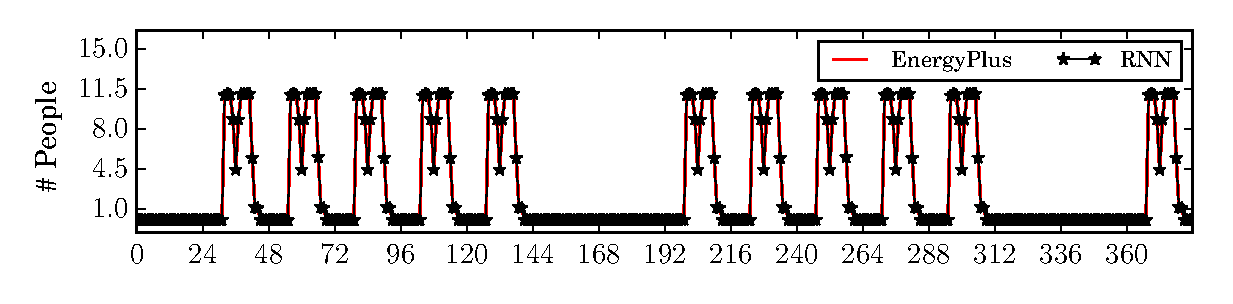
\includegraphics[width=0.45\columnwidth]{figs/results/1LAmbHVACDPFAugW3-4}
    }
    \caption{Occupancy estimation accuracy using one-layer recurrent neural network with input configuration I and II.}
    \label{fig:one-layer}
\end{figure*}

\begin{figure*}[htb]
    \centering
    \subfloat[Conf. I: Ambient factors and room temperatures]{
        \includegraphics[width=0.45\columnwidth]{figs/results/2LRoomTOnlyDPFAugW3-4}
    }
    \subfloat[Conf. II: Ambient factors, room temperatures and HVAC powers]{
        \includegraphics[width=0.45\columnwidth]{figs/results/2LAmbHVACDPFAugW3-4}
    }
    \caption{Occupancy estimation accuracy using two-layer recurrent neural network with input configuration I and II.}
    \label{fig:two-layer}
\end{figure*}

The training and validation error statistics are shown in
Table~\ref{tab:terr-stat} and Table~\ref{tab:verr-stat}, respectively.
In the input configuration I, we use ambient and room temperatures
only as the inputs (this is similar to situation in which we only know
temperature information from thermal sensors); in the input
configuration II, we use ambient, room temperatures and HVAC
cooling/heating powers as the inputs (in case we know more information
about a building).  

At every sample point, estimation error $e_i$ is calculated using
$e_i=\left|p_i^{\text{RNN}}-p_i^{\text{EP}}\right|$, where
$p_i^{\text{RNN}}$ is people occupancy estimated by the RNN and
$p_i^{\text{EP}}$ is referencing value used in \EP{}. Note that we may
have zero people in a room (so the occupancy value $p_i^{EP} = 0$), so
no relative errors are used. Also, occupancy values can be
non-integer numbers as the estimated number of people in a room is a
average number in a period.

In Table~\ref{tab:terr-stat} and Table~\ref{tab:verr-stat}, average
error is calculated using $\frac1n\sum_ne_i$; maximum error is
calculated using $\max\{e_i\}$; error rate is the number of points
where $e_i>0.5$. We discuss the estimation accuracy separately about
data configuration I and II.

\begin{table}[t]
    \centering
    \begingroup
    \setlength{\tabcolsep}{3.6pt} % Default 6pt
    \begin{tabular}{lrrcrrcrr}
        \toprule
        & \multicolumn{2}{c}{1 Hidden Layer} && \multicolumn{2}{c}{2 Hidden Layers} && \multicolumn{2}{c}{3 Hidden Layers}\\
        \cmidrule{2-3} \cmidrule{5-6} \cmidrule{8-9}
        & Conf.~I & Conf.~II && Conf.~I & Conf.~II && Conf.~I & Conf.~II\\
        \midrule
        Avg.~error & 0.451      & 0.0149    && 0.00635   & 0.00643   && 0.0308      & 0.0291    \\
        Max.~error & 12.6       & 0.544     && 0.284     & 0.141     && 0.807       & 0.788     \\
        Error rate & 20\%       & 0.0061\%  && 0.00\%    & 0.00\%    && 0.082\%     & 0.015\%   \\
        \bottomrule
    \end{tabular}
    \endgroup
    \caption{Training error statistics of three Elman architectures using two
        different input configurations.}
    \label{tab:terr-stat}
\end{table}

\begin{table}[t]
    \centering
    \begingroup
    \setlength{\tabcolsep}{3.6pt} % Default 6pt
    \begin{tabular}{lrrcrrcrr}
        \toprule
        & \multicolumn{2}{c}{1 Hidden Layer} && \multicolumn{2}{c}{2 Hidden Layers} && \multicolumn{2}{c}{3 Hidden Layers}\\
        \cmidrule{2-3} \cmidrule{5-6} \cmidrule{8-9}
        & Conf.~I & Conf.~II && Conf.~I & Conf.~II && Conf.~I & Conf.~II\\
        \midrule
        Avg.~error & 0.538      & 0.0175    && 0.153     & 0.00560   && 0.0439      & 0.0340    \\
        Max.~error & 17.8       & 2.82      && 18.1      & 0.288     && 11.4        & 1.66      \\
        Error rate & 21\%       & 0.11\%    && 2.4\%     & 0.00\%    && 0.71\%      & 0.38\%    \\
        \bottomrule
    \end{tabular}
    \endgroup
    \caption{Validation error statistics of three Elman architectures using two
        different input configurations.}
    \label{tab:verr-stat}
\end{table}

In data configuration I, one-layer network suffers from under-fitting
problem (about 20\% data points have errors greater than 0.5). This is
because the network needs more internal status to have the capability
to estimate the people occupancy only use room and ambient
temperature.  As we increasing the number of network layers,
estimation accuracy improves (error rate 2.4\% for 2-layer and 0.71\%
for 3-layer). Experiment results show that the RNN is able to estimate
people occupancy only with ambient and room temperatures with a good
accuracy (lower than 1\%).

In the configuration II, we provides more information (HVAC powers)
for the occupancy training process than the configuration I. As a
result, the ELNN with only two hidden recurrent layers can
already perform quite well (no points having error grater than 0.5
were observed in the one-year data). As network size grows (up to 3),
the estimation error grows (0.38\%), but stays in acceptable level.
